\section{Problem Definition}
\label{sec:problem}

\begin{definition}
\label{def:mention}
A {\em mention table} $T_M$ is a tuple $(\textbf{m}, P, L_1)$, where:
$\textbf{m}$ is a matrix of mentions and $\textbf{m}_{ij}$ represents a specific cell in table at $i^{th}$ row and $j^{th}$ column;
$P$ is a set of indices $\langle i,j  \rangle$ indicating $\underline{P}$osition of cells needs to be linked;
$L_1$ is the language in which table mentions $\textbf{m}$ are written.
\end{definition}

\begin{definition}
	A {\em Knowledge Base} $K$ is a tuple $(E, L_2)$, where:
	$E$ is a finite set of unique entities in $KB$;
	$L_2$ is the language in which $KB$ is written.
\end{definition}

\begin{definition}
An {\em entity table} $T_E$ is a tuple $(\textbf{e}, P, L_2)$, where:
$\textbf{e}$ is a matrix of entities and $\textbf{e}_{ij} \in E$ represents a specific cell in table at $i^{th}$ row and $j^{th}$ column;
$P$ is a set of indices $\langle i,j  \rangle$ indicating $\underline{P}$osition of cells have been linked;
$L_2$ is the language in which linked entities $\textbf{e}$ are written.
\end{definition}

\begin{definition}
Cross-lingual table linking seeks to find a mapping $\mathcal{F}$ between a mention table $T_M$ and an entity table $T_E$, so that each mention $\textbf{m}_{ij}$ where $\langle i,j\rangle \in M$ is linked to a corresponding entity $\textbf{e}_{ij}$.
\end{definition}

In practice, many web tables contain unlinkable entities such as numbers, dates
and times. There are some existing work that deals with the identification of
such numerical or temporal entities in Web Tables\cite{sun2015modeling}. 
In this paper, we assume that all the web tables have been preprocessed to 
remove all unlinkable columns (or rows), and as a result, every cell in the input table can be linked, unless the knowledge base doesn't contain the corresponding entity, which is shown as grey cell in \figref{fig:problem}. All the red cells in mention table will be linked to corresponding purple cells in entity table.

 
\begin{figure}[th]
	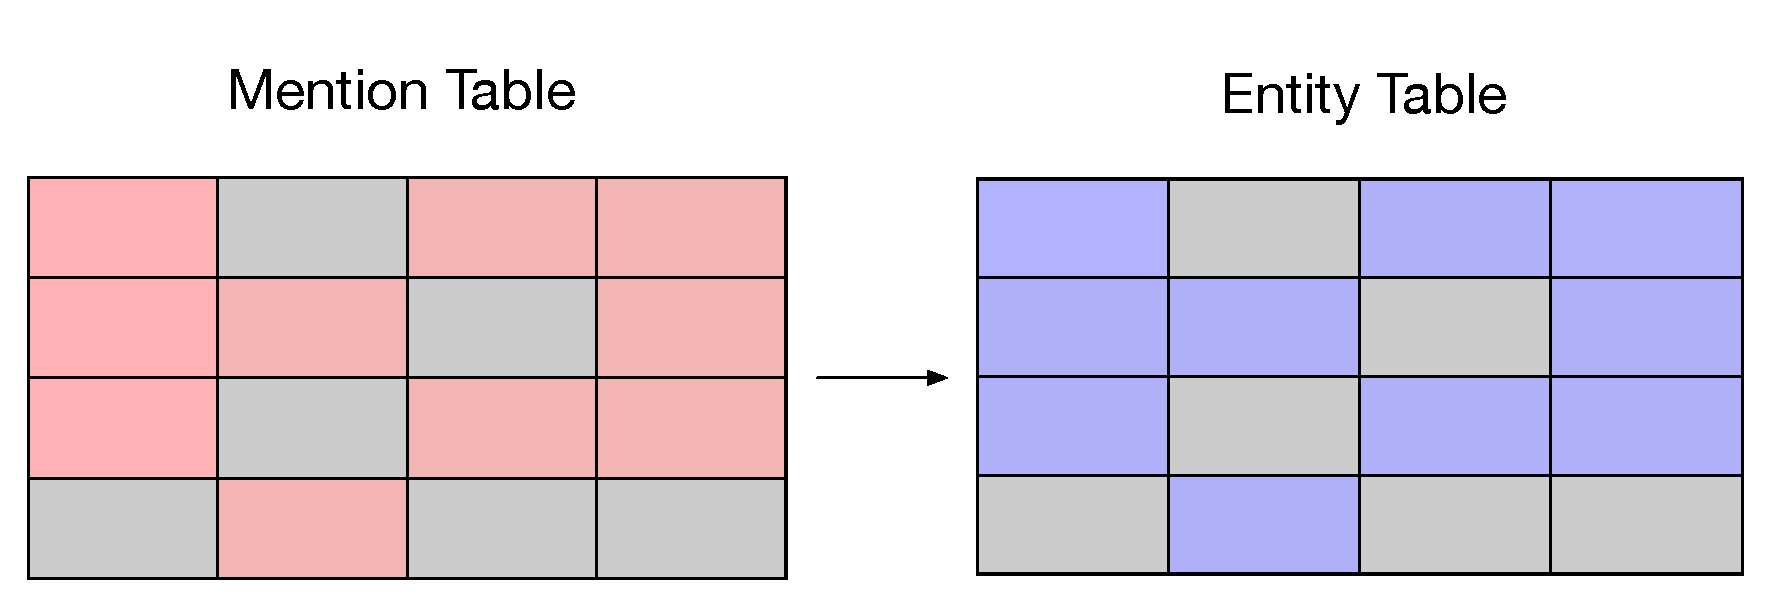
\epsfig{file=problem.eps, angle=0, width=1.0\columnwidth}
	\caption{Snapshot of cross-lingual table linking}
	\label{fig:problem}
\end{figure}

